\documentclass{beamer}
\usetheme{Madrid}
\usecolortheme{default}
\useoutertheme{split}
\useinnertheme{circles}
\usepackage{xcolor}
\usepackage{mathrsfs}
\usepackage{amsmath}
\usepackage{amssymb}
\usepackage{booktabs}
\usepackage{hyperref}
\usepackage{animate}
\usepackage{caption}
\usepackage{tikz}
\usetikzlibrary{arrows.meta, positioning, shapes.geometric, shadows}
\captionsetup[figure]{font=tiny}

\usepackage[
    backend=biber,
    style=alphabetic,
    sorting=ynt
]{biblatex}
\addbibresource{bibliography.bib}

% --- Couleurs CS ---
\definecolor{CSred}{RGB}{160,32,60}
\definecolor{CSgrey}{RGB}{136,121,150}
\definecolor{UPSred}{RGB}{97,21,58}
\setbeamercolor{titlelike}{bg=CSred}
\setbeamerfont{title}{series=\bfseries}
\setbeamercolor{palette primary}{bg=CSred,fg=white}
\setbeamercolor{palette secondary}{bg=CSred,fg=white}
\setbeamercolor{palette tertiary}{bg=CSgrey,fg=white}
\setbeamercolor{palette quaternary}{bg=CSgrey,fg=white}
\setbeamercolor{structure}{fg=CSgrey}

\title[Détection de Manipulation]{Détection Probabiliste de Manipulation de Marchés}
\subtitle{Soutenance Intermédiaire 2 - Projet de Recherche}
\author[Jamal, Martini]{Adonis~Jamal \and Jean Martini\\Encadrant : Damien Challet}
\institute[CentraleSupélec]{CentraleSupélec -- Laboratoire MICS}
\date[16 février 2026]{16 février 2026}

\titlegraphic{
    
\includegraphics[height=0.8cm]{img/logo_cs}
    \hspace{2cm}
    
\includegraphics[height=0.8cm]{img/logoMICS.png}
}

\begin{document}

\frame{\titlepage}

\begin{frame}
    \frametitle{Sommaire}
    \tableofcontents
\end{frame}

% ==============================================================================
% SECTION 1: INTRODUCTION
% ==============================================================================
\section{Introduction}
\subsection{Rappel du Contexte}
\begin{frame}{Le défi de la détection de spoofing}
    \begin{block}{Le Mécanisme}
        \begin{itemize}
            \item \textbf{Action :} Placer des ordres massifs non-bona fide loin du prix.
            \item \textbf{But :} Créer une illusion de pression pour manipuler les algorithmes.
            \item \textbf{Signal :} Dépendance forte à la distance au mid-price et au flux d'ordres \cite{tao_2020}.
        \end{itemize}
    \end{block}
    \begin{alertblock}{Verrous Scientifiques}
        \begin{enumerate}
            \item \textbf{Absence de Vérité Terrain :} Pas de labels "Manipulé / Non Manipulé".
            \item \textbf{Non-stationnarité :} Le marché change de régime (volatilité, liquidité) en permanence.
            \item \textbf{Contamination :} Le jeu d'entraînement contient déjà des manipulations invisibles.
        \end{enumerate}
    \end{alertblock}
\end{frame}

\subsection{Objectifs et Avancement}
\begin{frame}{Trajectoire du projet}
    \textbf{Objectif final :} Une meilleure caractérisation de la "spoofability" des marchés, avec une comparaison entre actions et crypto.

    \vspace{0.2cm}
    \begin{enumerate}
        \item \textbf{Phase 1 : Modélisation (Oct - Déc)}
        \begin{itemize}
            \item Prise en main et exploration de l'état de l'art et des features.
            \item Construction des features (Hawkes Process \cite{fabre_2025}, LOB shape).
            \item Implémentation de modèles (PNN, Transformer+OCSVM \cite{poutre_2024}).
        \end{itemize}
        \item \textbf{Phase 2 : Détection Robuste (Jan - Fév)}
        \begin{itemize}
            \item Entraînement séquentiel pour gérer le drift.
            \item Gestion de la contamination (PRAE).
            \item Gestion du seuil de décision (EVT/DSPOT, FDR).
        \end{itemize}
        \item \textbf{Phase 3 : Interprétabilité \& Analyse (Mars - Avr)}
        \begin{itemize}
            \item Entraînement final avec Ruche.
            \item Interprétabilité (Integrated Gradients, Occlusion).
            \item Tests sur les données crypto et comparaison avec les actions.
        \end{itemize}
    \end{enumerate}
\end{frame}


% ==============================================================================
% SECTION 2: ÉTAT DE L'ART (BIBLIO)
% ==============================================================================
% \section{État de l'art}
% \subsection{Synthèse Bibliographique}
% \begin{frame}{État de l'art : briques utiles pour une détection robuste}
%     \begin{itemize}
%         \item \textbf{Un score d'anomalie} (non supervisé) : reconstruction AE, ou score One-Class \cite{poutre_2024}.
%         \begin{itemize}
%             \item Exemple : $E_t = \lVert x_t - \hat{x}_t \rVert_2^2$ ; un pic indique une dynamique inhabituelle.
%         \end{itemize}
% 
%         \item \textbf{Robustesse à la contamination du train set} : PRAE apprend à \textbf{ne pas} reconstruire les outliers \cite{lindenbaum2022prae}.
% 
%         \item \textbf{Décision sous drift} : EVT/DSPOT transforme un flux de scores en alertes avec \textbf{taux de faux positifs contrôlé} \cite{siffer:hal-01640325}.
% 
%         \item \textbf{Explicabilité} : Integrated Gradients (dérivable) \& Occlusion (boîte noire) pour relier alertes \rightarrow features \cite{sundararajan2017axiomaticattributiondeepnetworks}.
%     \end{itemize}
% \end{frame}


% ==============================================================================
% SECTION 3: MÉTHODOLOGIE
% ==============================================================================
\section{Méthodologie}
\subsection{Approche Globale}
\begin{frame}{Architecture du Pipeline de Détection}
    On couple un \textbf{générateur de score robuste} avec un \textbf{décideur adaptatif}.
    
    \vspace{0.2cm}
    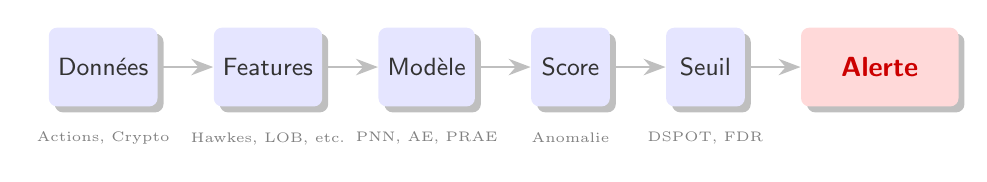
\begin{tikzpicture}[
        % Définition des styles pour une réutilisation facile
        node distance = 0.7cm, % Distance entre les blocs
        every node/.style = {font=\sffamily\small}, % Police sans-serif
        % Style des blocs standards
        block/.style = {
            rectangle, 
            draw=none, 
            fill=blue!10, 
            text=black!80, 
            minimum width=1cm, 
            minimum height=1cm, 
            rounded corners=3pt,
            drop shadow,
            align=center
        },
        % Style spécifique pour l'alerte (mise en évidence)
        alert/.style = {
            rectangle, 
            draw=none, 
            fill=red!15, 
            text=red!80!black, 
            minimum width=2cm, 
            minimum height=1cm, 
            rounded corners=3pt,
            drop shadow,
            align=center,
            font=\sffamily\bfseries
        },
        % Style des flèches
        arrow/.style = {
            -{Stealth[scale=1.2]}, % Pointe de flèche moderne
            thick, 
            draw=gray!50
        }
    ]

        % 1. Placement des nœuds (Nodes)
        \node (data)   [block] {Données};
        \node (feat)   [block, right=of data] {Features};
        \node (model)  [block, right=of feat] {Modèle};
        \node (score)  [block, right=of model] {Score};
        \node (thresh) [block, right=of score] {Seuil};
        \node (alert)  [alert, right=of thresh] {Alerte};

        % 2. Tracé des flèches (Arrows)
        \draw [arrow] (data) -- (feat);
        \draw [arrow] (feat) -- (model);
        \draw [arrow] (model) -- (score);
        \draw [arrow] (score) -- (thresh);
        \draw [arrow] (thresh) -- (alert);

        % 3. (Optionnel) Ajout de légendes ou annotations
        % Exemple : Annotation sous le seuil
        \node [below=0.2cm of data, font=\tiny, text=gray] {Actions, Crypto};
        \node [below=0.2cm of feat, font=\tiny, text=gray] {Hawkes, LOB, etc.};
        \node [below=0.2cm of model, font=\tiny, text=gray] {PNN, AE, PRAE};
        \node [below=0.2cm of score, font=\tiny, text=gray] {Anomalie};
        \node [below=0.2cm of thresh, font=\tiny, text=gray] {DSPOT, FDR};

    \end{tikzpicture}

    \begin{itemize}
        \item \textbf{Problème 1 (Apprentissage) :} Le jeu de données d'entraînement contient déjà des manipulations. Un Auto-Encodeur standard apprendrait à les reconstruire.
        \item \textbf{Solution 1 :} \textbf{PRAE}, Probabilistic Robust Auto-Encoder \cite{lindenbaum2022prae}.
        
        \vspace{0.1cm}
        \item \textbf{Problème 2 (Inférence) :} La distribution des erreurs de reconstruction change au cours du temps.
        \item \textbf{Solution 2 :} \textbf{DSPOT}, Drift Streaming Peaks-Over-Threshold \cite{siffer:hal-01640325}.
    \end{itemize}
\end{frame}

\subsection{Entraînement Robuste}
\begin{frame}{Entraînement robuste : PRAE}
    \textbf{Contexte :} L'historique contient des épisodes manipulés non étiquetés.

    \textbf{Idée :} Apprendre simultanément les paramètres du réseau $\theta$ et le "degré de normalité" $z_i$ de chaque échantillon $x_i$.

    \vspace{0.1cm}
    \begin{block}{Principe \cite{lindenbaum2022prae}}
        On apprend une variable latente $z_i \in [0,1]$ (inlierness) pour chaque échantillon $x_i$.
        \begin{itemize}
            \item $z_i \approx 1$ : \textbf{Inlier} (Donnée saine). Le modèle doit minimiser l'erreur de reconstruction.
            \item $z_i \approx 0$ : \textbf{Outlier} (Manipulation/Bruit). Le modèle doit ignorer cette donnée.
        \end{itemize}
    \end{block}

    Cela permet de "nettoyer" le dataset de manière endogène pendant l'entraînement, sans supervision externe.
\end{frame}

\begin{frame}{PRAE : Formulation Mathématique}
    On peut décrire la fonction de coût par rapport au poids $\psi, \rho$ du réseau et des variables latentes $z_i$ : $$L_{p_n}(\psi, \rho, \mu) = \mathbb{E}\left( \sum_i z[i] \left\|x_i - \hat{x}_i\right\|_2^2 - \lambda \|z\|_n  \right),$$ avec $z[i] = \max\left(0, \min\left(1, \mu[i] + \epsilon[i]\right)\right), \quad \epsilon[i] \sim \mathcal{N}(0, \sigma^2)$.

    \vspace{0.3cm}
    \begin{itemize}
        \item \textbf{Rôle de $\lambda$ :} Contrôle la quantité de données rejetées.
        \begin{itemize}
            \item Si l'erreur $\| x_i - \hat{x}_i \|^2 > \lambda$, il est optimal de mettre $z_i = 0$.
            \item $\lambda$ agit comme un seuil implicite de robustesse.
        \end{itemize}
    \end{itemize}
    
    Le vecteur $\mu$ sert de score d'anomalie pour chaque échantillon : plus $\mu_i$ est petit, plus $x_i$ est considéré comme un outlier.
\end{frame}

\subsection{Définition du Seuil et Décision}
\begin{frame}{DSPOT : Théorie des Valeurs Extrêmes (EVT)}
    Une fois le modèle entraîné, nous obtenons un flux de scores d'anomalie $e_t$. Il faut définir un seuil de décision pour déclencher une alerte.
    
    \begin{block}{Hypothèse EVT (Pickands-Balkema-De Haan)}
        Pour une large classe de distributions, la distribution des excès $y = e_t - u$ au-dessus d'un seuil élevé $u$ converge vers une Loi de Pareto Généralisée (GPD) :
        $$ G_{\gamma, \sigma}(y) = 1 - \left( 1 + \frac{\gamma y}{\sigma} \right)^{-1/\gamma} $$
    \end{block}
    
    Cela nous permet d'estimer la probabilité d'événements rares ("Queue de distribution") sans connaître la distribution complète des données (souvent inconnue et complexe).
\end{frame}

\begin{frame}{DSPOT : Algorithme de seuillage dynamique}
    \begin{block}{Calcul du seuil d'alerte $z_q$}
        Pour un risque cible $q$ (ex: $10^{-4}$), le seuil $z_q(t)$ est donné par l'inversion de la GPD : $$ z_q(t) = u + \frac{\sigma_t}{\gamma_t} \left[ \left( \frac{q N_w}{N_u} \right)^{-\gamma_t} - 1 \right] $$
    \end{block}
    
    \begin{itemize}
        \item $\sigma_t, \gamma_t$ : Paramètres d'échelle et de forme (estimés par MLE sur les pics récents).
        \item $N_w$ : Taille de la fenêtre glissante.
        \item $N_u$ : Nombre de pics dans la fenêtre.
    \end{itemize}
    
    DSPOT met à jour les paramètres sur une fenêtre glissante pour s'adapter au changement de régime $\Rightarrow$ Si le marché devient très volatil, $\sigma_t$ augmente, donc le seuil $z_q(t)$ augmente automatiquement.
\end{frame}


% ==============================================================================
% SECTION 4: CONCLUSION
% ==============================================================================
\section{}
\begin{frame}{}
    \centering
    \LARGE{Merci pour votre attention}
\end{frame}


% ==============================================================================
% SECTION : BIBLIOGRAPHIE
% ==============================================================================
\begin{frame}[allowframebreaks]
    \frametitle{Bibliographie}
    \nocite{*}
    \printbibliography
\end{frame}


% ==============================================================================
% SECTION : ANNEXE
% ==============================================================================
\appendix
\section{Annexe}
\subsection{Contexte}
\begin{frame}{Le carnet d'ordres (LOB)}
    \frametitle{Les marchés et le Carnet d'Ordres}
    \begin{itemize}
        \item \textbf{Limit Order Book (LOB) :} Répertoire central des intentions d'achat (Bid) et de vente (Ask).
        \item \textbf{Dynamique :} Le prix médian (\textit{mid-price}) réagit à l'état instantané et au flux d'ordres passé (Order Flow).
        \item \textbf{Données :} 
        \begin{itemize}
            \item Données Haute Fréquence (Level 2 / Market-by-order).
            \item Nécessité de traiter des millions d'événements par jour.
        \end{itemize}
    \end{itemize}
    \begin{block}{Problématique}
        La microstructure du marché peut être exploitée pour induire les autres participants en erreur.
    \end{block}
\end{frame}

\begin{frame}{Le spoofing}
    \frametitle{Le spoofing : une manipulation structurelle}
    \begin{itemize}
        \item \textbf{Définition :} Placer des ordres non-bona fide (sans intention d'exécution) pour créer une fausse impression de liquidité ou de pression directionnelle.
        \item \textbf{Tactiques courantes :}
        \begin{itemize}
            \item \textit{Layering :} Empilement d'ordres à différents niveaux de prix.
            \item \textit{Vacuuming :} Création de vides de liquidité pour provoquer des mouvements brusques.
        \end{itemize}
        \item \textbf{Mécanisme :} 
        \begin{enumerate}
            \item Placer un gros ordre d'achat (Fake) loin du prix.
            \item Attendre que le prix monte (réaction des algos).
            \item Vendre réellement (Bona fide) à un prix plus élevé.
            \item Annuler l'ordre d'achat initial.
        \end{enumerate}
    \end{itemize}
\end{frame}

\subsection{Hypothèses}
\begin{frame}{Hypothèses de travail}
    \begin{block}{Hypothèses Microstructurelles}
        \begin{itemize}
            \item La distance de placement des ordres limites joue un rôle critique dans la formation des prix (contrairement aux modèles basés uniquement sur le volume au best bid/ask) \cite{tao_2020}.
            \item Un agent manipulateur agit rationnellement pour minimiser son coût d'exécution espéré.
        \end{itemize}
    \end{block}

    \begin{block}{Hypothèse Comparative}
        En l'absence de régulation stricte, les carnets d'ordres de crypto-monnaies (CEX) présentent :
        \begin{itemize}
            \item Une fréquence de spoofing plus élevée.
            \item Une sensibilité (impact prix) plus forte aux ordres de spoofing que les marchés actions traditionnels.
        \end{itemize}
    \end{block}
\end{frame}



\subsection{Entraînement et Interprétabilité}
\begin{frame}{Entraînement séquentiel}
    \frametitle{Entraînement séquentiel}
    \begin{block}{Pourquoi séquentiel}
        Les distributions de features et de scores dérivent (liquidité/volatilité/régimes). Un entraînement "one-shot" généralise mal.
    \end{block}

    \begin{block}{Stratégie explorée}
        \begin{enumerate}
            \item \textbf{Entraînement} sur une période de 1 heure, divisée en blocs d'entraînement et de validation (3 à 6 blocs).
            \item \textbf{Fine-tuning} jour après jour avec early stopping.
            \item \textbf{Tests} sur un nouveau jour avec distinction entre matin et restant de la journée.
        \end{enumerate}
    \end{block}
\end{frame}

\begin{frame}{Integrated Gradients}
    \frametitle{Integrated Gradients pour l'Interprétabilité}
    \textbf{Objectif :} attribuer la contribution des features à un score (log-vraisemblance, erreur, etc.) pour les modèles \textbf{dérivables}.

    \begin{block}{Principe}
        On compare une entrée $x$ à une baseline $x'$ et on intègre les gradients le long du chemin $x' \rightarrow x$ :
        \[
        \mathrm{IG}_i(x)=(x_i-x'_i)\int_{0}^{1}\frac{\partial f\big(x' + \alpha(x-x')\big)}{\partial x_i}\,d\alpha
        \]
    \end{block}
\end{frame}

\begin{frame}{Occlusion Sensitivity}
    \frametitle{Occlusion Sensitivity pour l'Interprétabilité}
    \textbf{Objectif :} interpréter des modèles \textbf{non-dérivables} (ex : One-Class SVM) ou obtenir une explication modèle-agnostique.

    \begin{block}{Principe}
        On masque (occlusion) un sous-ensemble de variables (ou un groupe : échelle de temps, distance, côté bid/ask) et on observe la variation du score :
        \[
        \Delta s = s(x) - s\big(\mathrm{mask}(x,\mathcal{G})\big)
        \]
        Une grande chute du score signifie que le groupe $\mathcal{G}$ est important.
    \end{block}
\end{frame}


\end{document}